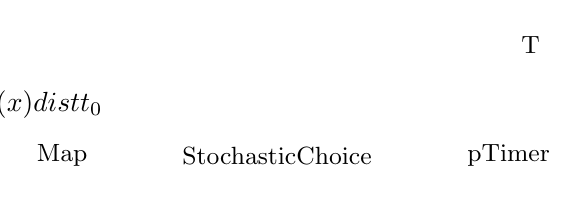
\begin{tikzpicture}[scale=1.4]

\tikzstyle{every node}=[font=\small]
\tikzstyle{label}=[draw=none]

\draw (0.75, -0.4) node[label] {Map};
\draw (2.7, -0.4) node[label] {StochasticChoice};
\draw (4.8, -0.4) node[label] {pTimer};

\draw (5, 0.6) node[label] {T};

\map{(0,0)}{(1.5,0)}{node [above=3] {$f(x)$}}
\choice{(1.95,0)}{(3.45,0)}{node [above=0.2cm, xshift=-0.6cm] {$dist$}}
\ptimer{(4.1,0)}{(4.85, 0.6)}{(5.6,0)}{node [above=1, xshift=-0.2cm] {$t_0$}}

\end{tikzpicture}